\begin{frame}{Canonical search problem $\Search_{\varphi}$ (Impagliazzo et al. 1994)}

	
    $\varphi(x, y)$ is an unsatisfiable CNF formula:
    \begin{itemize}
        \item Alice receives a substitution to the variables $x$, Bob receives a substitution to the
            variables $y$;
        \item goal is to find a clause $C \in \varphi$ that is unsatisfied by this substitution.
    \end{itemize}

    \pause

    \begin{theorem}[Beame, Pitassi, Segerlind 2007. Informal]
        If there is a {\color{blue} tree-like} proof in proof system $\Pi$ ($\Pi$ from some \textit{huge
          class}) of size $S$ then there is a communication protocol for $\Search_{\varphi}$ of depth
        $poly(\log(S))$.
    \end{theorem}
    
\end{frame}


\begin{frame}{Proofs and games}
	$D_1, D_2, \dots, D_{17}$ is a semantic proof of of $\varphi(x, y)$.

    \begin{center}
    	\tikzstyle{inner} = [thin, circle, minimum size = 0.6cm, draw, inner sep = 0.1pt, black, font = \scriptsize]
\tikzstyle{inner_g} = [thin, circle, minimum size = 0.6cm, draw, inner sep = 0.1pt, black, fill = green]
\tikzstyle{inner_r} = [thin, circle, minimum size = 0.6cm, draw, inner sep = 0.1pt, black, fill = red]
\tikzstyle{inner_b} = [
	thin, circle, minimum size = 0.6cm, draw, inner sep = 0.1pt, black, fill = blue!30!white, font =
    \scriptsize]
\tikzstyle{ed} = [thick, ->, draw, black]

    
\begin{tikzpicture}

    \only<-1>{
        \node[inner] (a) at (0, 0) {$D_{17}$};
	}
    \only<2->{
        \node[inner_b] (a) at (0, 0) {$D_{17}$};
    }

    \only<-2>{
        \node[inner] (b) at (-1.5, -1) {$D_{16}$};
	}
    \only<3->{
        \node[inner_b] (b) at (-1.5, -1) {$D_{16}$};
    }
  

    \node[inner] (c) at (1.5, -1) {$D_{15}$};

    \node[inner] (d) at (-3, -2) {$D_{14}$};

    \only<-3>{
        \node[inner] (e) at (0, -2) {$D_{13}$};
	}
    \only<4->{
        \node[inner_b] (e) at (0, -2) {$D_{13}$};
    }

    \node[inner] (f) at (3, -2) {$D_{12}$};

    \node[inner] (g) at (-4.5, -3) {$D_{11}$};

    \only<-4>{
        \node[inner] (h) at (-1.5, -3) {$D_{10}$};
	}
    \only<5->{
        \node[inner_b] (h) at (-1.5, -3) {$D_{10}$};
    }

    \node[inner] (i) at (1.0, -3) {$D_9$};

    \only<-6>{
        \node[inner] (j) at (2.0, -3) {$D_8$};
	}
    \only<7->{
        \node[inner_b] (j) at (2.0, -3) {$D_8$};
    }

    \node[inner] (k) at (4.0, -3) {$D_7$};

    \only<-5>{
        \node[inner] (l) at (-2.5, -4) {$D_6$};
	}
    \only<6->{
        \node[inner_b] (l) at (-2.5, -4) {$D_6$};
    }

    \node[inner] (m) at (-0.5, -4) {$D_5$};

    \only<-7>{
        \node[inner] (n) at (1.2, -4) {$D_4$};
	}
    \only<8->{
        \node[inner_b] (n) at (1.2, -4) {$D_4$};
    }

    \node[inner] (o) at (2.8, -4) {$D_3$};

    \node[inner] (p) at (0.4, -5) {$D_2$};
    
    \only<-8>{
        \node[inner] (q) at (2, -5) {$D_1$};
	}
    \only<9->{
        \node[inner_b] (q) at (2, -5) {$D_1$};
    }


    
    \path (a) edge[ed] (b);
    \path (a) edge[ed] (c);
    \path (b) edge[ed] (d);
    \path (b) edge[ed] (e);
    \path (c) edge[ed] (e);
    \path (c) edge[ed] (f);
    \path (d) edge[ed] (g);
    \path (d) edge[ed] (h);
    \path (e) edge[ed] (h);
    \path (e) edge[ed] (i);
    \path (f) edge[ed] (j);
    \path (f) edge[ed] (k);
    \path (h) edge[ed] (l);
    \path (h) edge[ed] (m);
    \path (j) edge[ed] (n);
    \path (j) edge[ed] (o);
    \path (n) edge[ed] (p);
    \path (n) edge[ed] (q);
\end{tikzpicture}    
    \end{center}

    \pause
    \pause
    \pause
    \pause
    \pause
    \pause
    \pause
    \pause
    \pause
    Size of game is the size of graph. Communication complexity of game is the communication complexity
    of evaluation of constaint.

\end{frame}

\begin{frame}{Plan [Kraj{\'{\i}}{\v{c}}ek 95]}

    \begin{enumerate}
        \item Proof in some proof system $\Rightarrow$ communication game for $\Search_{\varphi}$
            problem.
        \item Communication game for $\Search_{\varphi}$ problem $\Rightarrow$ communication game for
            $\MBit$ relation.
        \item Communication game for $\MBit$ relation $\Rightarrow$ monotone circuit for separator.
    \end{enumerate}
\end{frame}


\begin{frame}{Games and circuits}

    A communication problem on sets $U, V \subseteq \{0, 1\}^{n}$ and relation $\Bit$:
    \begin{itemize}
        \item Alice receives $u \in U$, Bob receives $v \in V$;
        \item goal is to find $i$ such that $u_i \neq v_i$.
    \end{itemize}
    \pause
    Monotone case ($\MBit$ relation):
    \begin{itemize}
        \item goal is to find $i$ such that $u_i = 1 \land v_i = 0$.
    \end{itemize}

    \pause

    \vspace{0.2cm}
    $U = f^{-1}(1), V = f^{-1}(0)$

    \begin{itemize}
        \item {[Karchmer, Wigderson 1990]} Communication protocol of size $S$ for the relation $\Bit$
            \alert{$(\MBit)$} $\Leftrightarrow$ \alert{(monotone)} boolean formula for $f$ of size $S$.
        \pause
        \item {[Razborov 94]} Communication game of size $S$ and $CC = k$ for the relation $\Bit$
            \alert{$(\MBit)$} $\Leftrightarrow$ \alert{(monotone)} boolean circuit for $f$ of size $2^k
            S$.
    \end{itemize}
\end{frame}

\begin{frame}{Results}
    \begin{itemize}
        \item {[Karchmer, Wigderson 1990]} Communication protocol of size $S$ for the relation $\Bit$
            \alert{$(\MBit)$} $\Leftrightarrow$ \alert{(monotone)} boolean formula for $f$ of size $S$.
        \item {[Razborov 94]} Communication game of size $S$ and $CC = k$ for the relation $\Bit$
            \alert{$(\MBit)$} $\Leftrightarrow$ \alert{(monotone)} boolean circuit for $f$ of size
            $2^{3k} S$.
        \pause
        \item {[Pudl{\'{a}}k 10, S 17]} Communication game of size $S$ and $CC = k$ for some relation $N$
            $\Leftrightarrow$ communication game of size $2^{3k} S$ and $CC = \frac{3}{2}$ (two
            independent rounds) for some relation $N$.
    \end{itemize}
    
    \vspace{0.3cm}
    \pause
    \begin{itemize}                
        \item {[S 17]} There are two $\NP$ sets such that any communication game of size $S$ and $RCC = 1$
            for the relation $\MBit$ has size at least $2^{n^{\frac{1}{8}}}$.
        \pause    
        \item {[Hrube{\v{s}}, Pudl{\'{a}}k 17]} Communication game of size $S$ and $RCC = 1$ for the
            relation $\MBit$ $\Leftrightarrow$ monotone {\color{blue} real}
            circuit for $f$ of size $O(S)$.
    \end{itemize}
\end{frame}


\begin{frame}{Plan [Kraj{\'{\i}}{\v{c}}ek 95]}

    \begin{enumerate}
        \item Proof in some proof system $\Rightarrow$ communication game for $\Search_{\varphi}$
            problem.
        \item Communication game for $\Search_{\varphi}$ problem $\Rightarrow$ communication game for
            $\MBit$ relation.
        \item Communication game for $\MBit$ relation $\Rightarrow$ monotone circuit for separator.
    \end{enumerate}
\end{frame}


\begin{frame}{$\MBit \le \Search_{\varphi}$}
    $U, V \in \{0, 1\}^n$ are disjoint $\NP$ sets:
    \begin{itemize}
        \item $\One(x, q)$ is a resonable encoding of the fact that $x \in U$;
        \item $\Zero(x, r)$ is a resonable encoding of the fact that $x \in V$;
        \item $\One(x, q) \land \Zero(x, r)$ is the unsatisfiable formula.            
    \end{itemize}

    \vspace{0.2cm}
    \pause
    Alice knows $u \in U$ and generates $q^u$ such that $\One(u, q^u)$ is satisfied. Bob knows $v \in
    V$ and generates $r^v$ such that $\Zero(v, r^v)$ is satisfied.

    \vspace{0.2cm}
    Reduction: $u, v \Rightarrow (u, q^u), r^v$ 

	\pause
    
    \begin{itemize}
        \item $C$ is not satisfied by $(u, q^u, r^v)$ $\Rightarrow$ $C \in \Zero(x, r)$;
        \pause
        \item $C$ is not satisfied by $r^v$ but $C$ is satisfied by $(v, r^v)$ $\Rightarrow$ $C = \neg
            x_i \lor D(r)$;
        \pause
        \item $u_i = 1$ and $v_i = 0$.   
    \end{itemize}
\end{frame}


\begin{frame}{$\MBit \le \Search_{\varphi}$}

    \begin{theorem}[Hrube{\v{s}}, Pudl{\'{a}}k 17; Fleming, Pankratov, Pitassi, Robere 17]
        For any unsatisfiable formula $\varphi$ there are two $\NP$ sets $U_{\varphi}, V_{\varphi}
        \subseteq \{0, 1\}^{\ell}$ such that:
        \begin{itemize}
            \item $U_{\varphi} \cap V_{\varphi} = \emptyset$;
            \item any protocol (game) that solves $\Search_{\varphi}$ also solves $\MBit$ relation on
                sets $U_{\varphi}, V_{\varphi}$.
        \end{itemize}
    \end{theorem}

    \begin{corollary}
        Random $\log(n)$-CNF and $\lang{BPHP}$ require an exponential proof in $\CP$.
    \end{corollary}
\end{frame}


\begin{frame}{Randomized games}

    \begin{itemize}
        \item $\ResL$ is a semantic proof system that operates with dijunctions of linear equation modulo
            $2$.
        \pause    
        \item Open problem: is there an explicit formula that requires superpolynomial proof in $\ResL$?
        \pause
        \item There is no small deterministic communication protocol for evaliation of constraints of
            $\ResL$. But there is a small randomized communication protocol.
        \pause
        \item Open problem: is there an explicit formula $\varphi$ such that any game for
            $\Search_{\varphi}$ with randomized communication complexity $O(1)$ requires superpolynomial
            size?
        \pause
        \item {[Kraj{\'{\i}}{\v{c}}ek 16]} Randomized games \alert{$\Rightarrow$} boolean circuits with
            local oracles.
        \pause
        \item {[Kraj{\'{\i}}{\v{c}}ek, I. Oliveira 17]} Conditional lower bounds on circuits with local
            oracles.
    \end{itemize}
\end{frame}


\begin{frame}{Open problems}
    \begin{enumerate}
            
        \pause
        \item Lower bound on boolean dag-like games for $\Search_{\varphi}$ for Tseitin formulas with small
            gadgets.
        \pause
        \item Lower bound on dag-like games with new validity condition: $A(h, x) = B(h, y)$ (motivated
            by lower bounds for other proof systems).
        \pause
        \item Can we use information complexity for this protocols?
    \end{enumerate}
\end{frame}